\documentclass[fleqn]{jbook}
\usepackage{physpub}

\begin{document}

\begin{question}{専攻 問題4}{}

図1は粉末固体試料からのX線の回折像を撮影するための実験装置を,実際の装置の大
きさを無視して,その概略を定性的に理解できるように,概念的に描いたものである。
この装置を用いて,単純立方格子を持つ粉末結晶試料からのX線の回折像を撮影するこ
とを試みる。図2は,カメラの中でのX線の入射方向,X線の回折方向,,写真フ
ィルム,回折像の位置の間の関係を示したものである。$R$は試料から写真フィルム
までの距離で6.0cm,$S$は,写真フィルム上で,ビームストッパーの中心から回折像
までの距離である。

この実験に関し次の設問に答えよ。設問{\bf 1}では,AからGの部分に該当する言葉また
は文章を書け。但し,X線の波長は1.54\AA である。また,必要とあれば,末尾の表1
を用いよ。

\begin{subquestions}
\SubQuestion
撮影を始める前に,試料を試料台にのせて固定する。次に,実験室の配電板の
スイッチを入れる。X線管を(A)するために水を流してから,X線発生装置の電源のスイ
ッチをいれ,X線の強度を決めるために,X線管の(B)と(C)を設定する。次に,X線管の
シャッターを開けて,ビームストッパーの窓から内蔵されている(D)を見て,(E)を通
って細いX線ビームが,きちんと入射していることを確かめる。もしも(D)が(F)なら,
カメラ支持台を動かして,カメラの位置を調整する。カメラ位置の調整が終わったら,
ひとまず(G)を切り,カメラをカメラ支持台からはずし,写真フィルムをカメラに入れ
て,カメラ支持台に固定する。そして再び(G)を出して,回折像を撮影する。

\SubQuestion
解析の対象とすることができるような回折像の撮影が一回の試行で成功すると
は限らない。考えられる失敗の原因を二つあげよ。

\SubQuestion
 フィルムに記録される回折像の図を定性的に描け(回折像の形状が定性的にわ
かればよい)。この回折像は通常,何と呼ばれるか。

\SubQuestion
現像された写真フィルム上で中心にもっとも近い回折像に対する$S$の値として
3.3cmという値が得られた。これより,この結晶の格子定数を求めよ。

\SubQuestion
上の試料において,$S=5.9{\rm cm}$の位置にも回折像が認められた。これはど
の結晶面からの回折像か。結晶面の指数で示せ。

\begin{center}
表1\\
\begin{tabular}{cc}
$\sin 13.5^{\circ}=0.233$ & $27.0^{\circ}=0.471 \rm rad $\\
$\sin 15.8^{\circ}=0.273$ & $31.5^{\circ}=0.550 \rm rad $\\
$\sin 20.6^{\circ}=0.352$ & $41.2^{\circ}=0.719 \rm rad $\\
$\sin 25.4^{\circ}=0.429$ & $50.8^{\circ}=0.886 \rm rad $\\
$\sin 28.2^{\circ}=0.473$ & $56.4^{\circ}=0.983 \rm rad $\\
$\sin 30.3^{\circ}=0.505$ & $60.6^{\circ}=1.058 \rm rad $\\
$\sin 32.7^{\circ}=0.540$ & $65.4^{\circ}=1.141 \rm rad $\\
\end{tabular}
\end{center}

\begin{center}
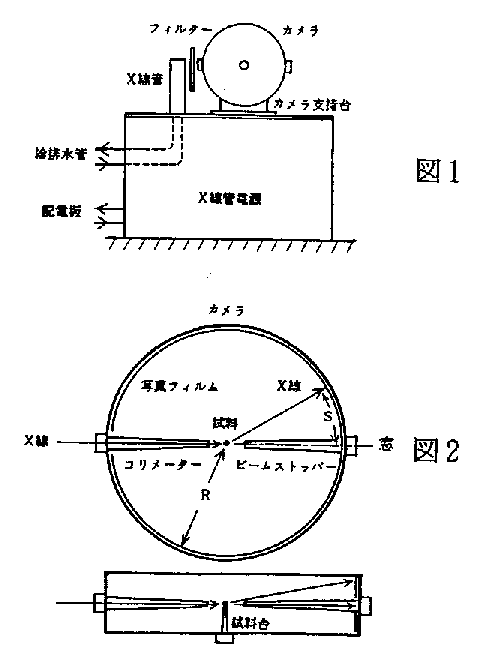
\includegraphics[clip]{1992phy4-1.eps}
\end{center}

\end{subquestions}
\end{question}
\begin{answer}{専攻 問題4}{}

\begin{subanswers}
\SubAnswer
\begin{itemize}
\item[A] \quad 冷却
\item[B] \quad 電圧
\item[C] \quad 電流(電圧の設定が先である)
\item[D] \quad 蛍光板(裸眼で見る人がたまにいるが危険である)
\item[E] \quad 試料
\item[F] \quad 光っていない
\item[G] \quad X線
\end{itemize}

\SubAnswer
1.X線が、試料の中心を通っていないため像がずれる、またはない。\\
2.X線の光量を間違う。または現像ミス。

\SubAnswer
デバイリング
\begin{center}
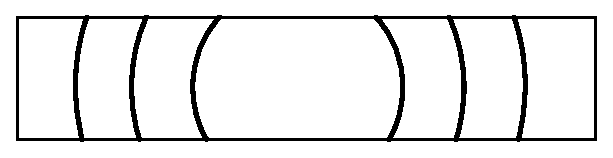
\includegraphics[clip]{1992phy4-2.eps}
\end{center}

\SubAnswer
$ S=3.3 \rm{cm}$ であるから、
\[ 2 \theta = \frac{3.3 {\rm cm}}{6 {\rm cm}} =0.55  [{\rm rad}] \]
\[ \theta =15.8^{\circ} \]
一方、$ S=3.3 \rm{cm}$ は最も中心に近い像であるから $n=1$ 。
よって
\[ d=2.82  \mbox{[\AA]} = a_0 \]

\SubAnswer
$S=5.9  \rm{cm}$ であるから、入射角は
\[ 2 \theta = \frac{5.9 \rm{cm}}{6 \rm{cm}} =0.983 [\rm{rad}] \]
\[ \theta =28.2^{\circ} \]
これと$2d \sin \theta =\lambda $ より
\[ d=1.63 \mbox{[\AA]} \]
となる。ここで面指数 $(h,k,l)$ に対して
\[ \frac{1}{d^2}=\frac{1}{a^2}(h^2+k^2+l^2) \]
の関係があるから、代入すると
\[ h^2+k^2+l^2 =3 \]
ゆえに
\[ (h,k,l)=(1,1,1) \]

\end{subanswers}
\end{answer}


\end{document}



